\documentclass{udpreport}
\title{Creación de paquetes utilizando Scapy y validación con
Wireshark}
\author{Integrantes: Francisca Carrrasco, Ignacio López, Nicolás Ramírez.\\Profesor: José Pérez
\\Ayudante: Alexis Inzunza}
\date{Mayo de 2017}
\usepackage{graphicx}
\graphicspath{ {Imagenes/} }
\udpschool{Escuela de Informática y Telecomunicaciones}

\begin{document}
\maketitle
\tableofcontents
\listoffigures
\chapter{Actividades}
	\section{Instalación de software}
    	El software ya estaba instalado, así que no fue necesario hacerlo. \\
	\section{Creación de Paquetes}
		Para comenzar con la creación de un paquete antes es necesario crear ciertas variables para definir de forma específica los campos de nuestro paquetito. Lo primero que debemos hacer es crear una variable y asignarle el comando “Ether()”, el cual trabaja en la segunda capa del modelo OSI (capa de enlace), después se la asigna un valor a la componente “dst” y “src”, estos valores son la MAC
		de destino y la de origen respectivamente.
		Después se crea otra variable a la cual se le asignará el comando “IP()”, el cual trabaja en la tercera
		capa del modelo OSI (capa de red), para esta variable se modificarán nuevamente las componentes “dst” y “src”, estas componentes corresponden a la IP de destino y a la de origen respectivamente.
		Posteriormente se crea una nueva variable y a esta se le asigna el
		comando “ICMP()” el cual trabaja en la cuarta capa del modelo OSI (capa de transporte). Continuando se crea otra variable y a esta se le asigna el comando “Raw()”, una vez hecho todo lo anterior se crea una nueva variable (nuestro paquete)  y se le asignan las variables anteriores separadas de un “/” en el mismo orden que fueron nombradas.
		
	\section{Switch}
		Existe una gran diferencia entre enviar paquetes en equipos conectados a un switch que enviarlos a equipos conectados a un HUB. A continuación se describirán los pasos llevados a cabo para enviar paquetes entre equipos conectados a un switch\\\\
		{\bf \large Envío Broadcast:}\\\\
		Lo que se hizo fue crear un paquete y en la variable que almacena el "Ether()", donde se pone hacia donde
		va dirigido (dst), se uso “ff:ff:ff:ff:ff:ff”, ya que era una transmisión de tipo broadcast.
		Finalmente se procede a enviar el paquete usando el comando “sendp“, ya que este comando sirve para enviar paquetes que van desde la segunda capa, una vez enviado el paquete se verifica que se haya recibido en todos los equipos que estábamos utilizando.\\\\
		
		{\bf \large Envío a otro equipo:}\\\\
		Para la creación de un paquete enviado a una dirección Mac específica, se modificó el "dst" a una dirección específica de
		Mac, Despues se volvió a crear el paquete como antes fue mencionado y usando el comando "sendp" fue enviado. Luego al revisar con wireshark se observa que
		efectivamente llega el paquete al equipo de destino.\\\\
		
		{\bf \large Envío MAC inexistente:}\\\\
		A continuación para enviar un paquete con la MAC errónea, se procede hacer los mismos procesos anteriormente
		mencionados,modificando la Mac de destino ("dst") a la de una que no este conectado a la res del laboratorio, luego se crea el paquete y se envia de la misma manera manera que las anteriores, con el comando "senp".
		Una vez enviado el paquete se procede a verificar en Wireshark, al observarlo nos damos cuenta de que el paquete enviado, al no encontrar la MAC de destino, procede a hacer una
		transmisión de tipo Broadcast y envía el paquete a todos los equipos conectados a la red.
		
		
		
	\section{HUB}
	 	Al mandar paquetes en la red por medio de un HUB estos paquetes siempre 
 		le llegaran a todos los dispositivos conectados a la red.Mientras que si
 		se mandaran paquetes como por intermedio de un switch estos dependerían de 
 		las direcciones de destino  y sus comandos característicos.\\
 		El HUB al hacer  los mismos procedimientos anteriores los cuales eran :\\
 		-Enviar paquete con MAC no existente en la red\\
 		-Enviar paquete con dirección MAC de destino FF:FF:FF:FF:FF:FF\\
 		-Enviar paquete a la MAC de un equipo en específico de la red\\
 		Este HUB repite el paquete hacia todos los dispositivos con cualquiera
 		de las formas anteriores realizadas en el switch.
 		
	\section{Cuestionario}
	
	  1.-¿Qué pasa cuando envío un paquete a la dirección FF:FF:FF:FF:FF:FF? ¿Quienes
	     lo reciben? ¿Por qué?\\
    	 	\begin{figure}[h]
	        	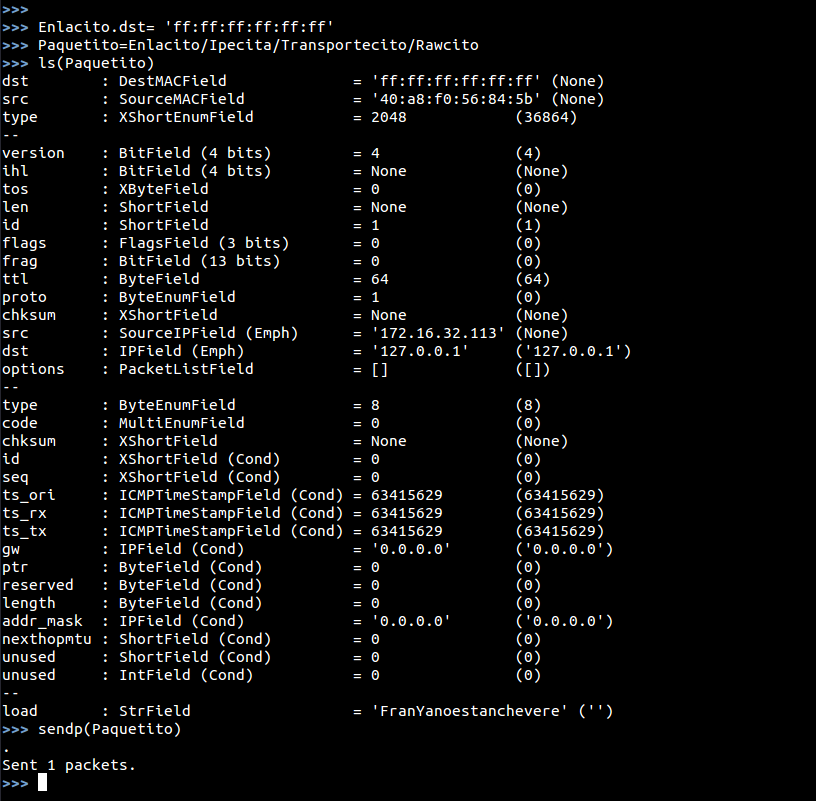
\includegraphics[width=10cm, height=11cm]{PaqueteMacConocida.png}
			\caption{Envío en Broadcast}
	        	% \label{fig:my_label}
	 	\end{figure}
	     Cuando enviamos un paquete a la dirección FF:FF:FF:FF:FF:FF, este fue enviado a todos los equipos dentro de la red
	     Ethernet. Esto es debido a que la dirección antes mencionada esta designada para que la difusión de nuestro paquete sea
 	     enviado a cada dispositivo conectado a nuestra red LAN, a este tipo de difusión se le conoce como “Broadcast”.\\
 	     \newpage
 
  	  2.-¿Qué pasa cuando envío un paquete a una MAC de otro equipo? ¿Quienes lo
  	      pueden recibir? ¿Por qué?\\
    		\begin{figure}[h]
  	          	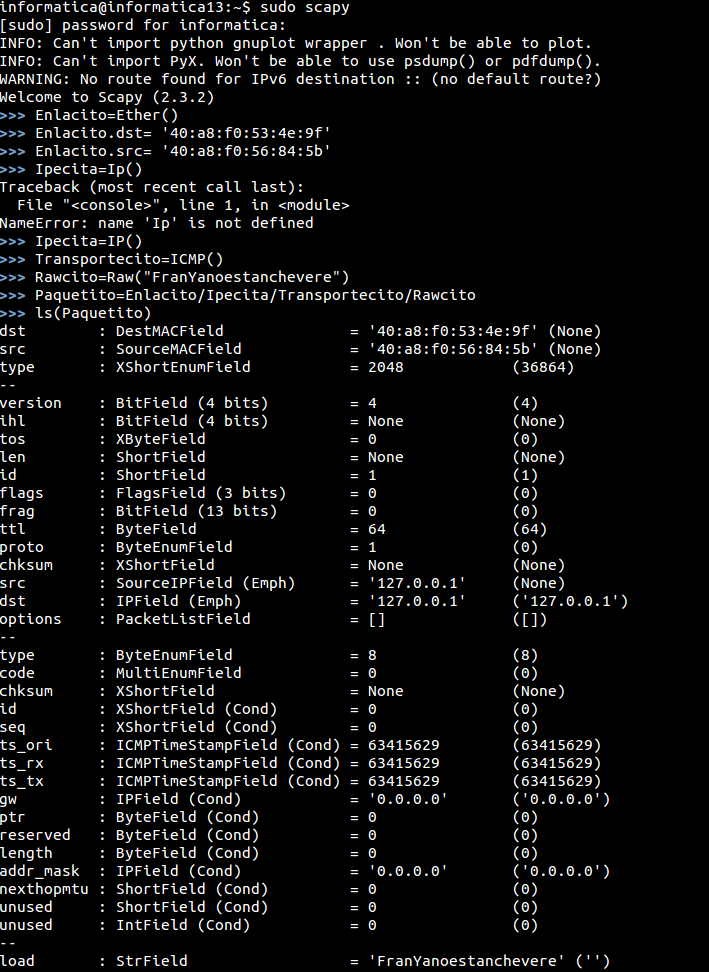
\includegraphics[width=10cm, height=11cm]{PaqueteOtraRed.png}
  	          	\caption{Envío a una MAC}
  	          	%\label{fig:my_label}
  		\end{figure}
 	      
 	      Cuando enviamos un paquete a la dirección MAC de otro equipo dentro de la red Ethernet, solamente el equipo que posee
 	      esa dirección es capaz de recibirlo. Esto ocurre puesto a que, como indicamos anteriormente, al paquete le dimos una
 	      MAC de destino fija, entonces el paquete se encargó de viajar solamente al equipo que poseía esa dirección\\
        \newpage
  	  3.-¿Qué sucede si envía un paquete a una MAC que no corresponda a ningún equipo
  	      de la red? ¿Quienes lo pueden recibir? ¿Por qué?\\
    		\begin{figure}[h]
  	          	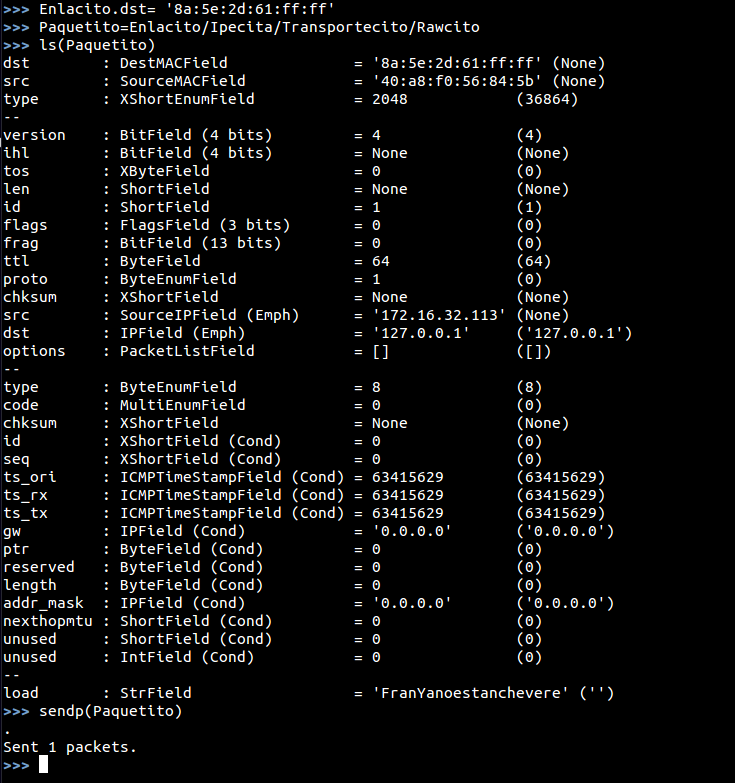
\includegraphics[width=10cm,height=11cm]{PaqueteMacMala.png}
  	        	\caption{Envío a una MAC fuera de la red}
  	            	%\label{fig:my_label}
  	        \end{figure}
 	      Cuando enviamos 
 	      Cuando enviamos un paquete a una dirección MAC que no correspondía a ningún equipo de la red, al enviarlo nos apareció
 	      el mensaje: “WARNING: Mac address to reach destination not found. Using Broadcast.” Y posteriormente el paquete fue
 	      enviado a todos los equipos pertenecientes a la red Ethernet. Se usa el Broadcast para así poder obtener todas las
 	      direcciones MAC mediante su IP, registrarlas en la lista ARP y encontrar la que se dio como destinataria, pero como esta
 	      no se encuentra en la red sigue mandando el paquete a todos los equipos que si están en la red para seguir buscando la
 	      MAC solicitada.\\

 	     
	      

\chapter{Conclusión}
  	      En esta experiencia de laboratorio se logra comprender cómo crear correctamente un paquete con Scapy,
  	      entendiendo todos sus componentes y cómo se puede enviar al o a los destinatarios que nosotros deseemos, también
  	      logra dejar clara la diferencia entre los comandos “send()” y “sendp()”, la capa en la que trabajan y cuando usar cada
  	      uno,se capta la forma en como funciona un Switch y un Hub con respecto al envío de paquetes y se aprendió trabajar con
  	      Wireshark para encontrar los paquetes del tipo que queramos o provenientes de la IP que cada uno  escoja.
\begin{thebibliography}{x}
\bibitem{Guide for Scapy} \textsc{Guide for Scapy},
\textit{https://theitgeekchronicles.files.wordpress.com/2012/05/scapyguide1.pdf}
\bibitem{Cisco Osi} \textsc{Cisco},
\textit{ http://www.cisco.com/cpress/cc/td/cpress/fund/ith/ith01gb.htm#xtocid166844}
\end{thebibliography}
\end{document}
